\documentclass{article}
\usepackage{arxiv}
\usepackage[utf8]{inputenc}
\usepackage[english, russian]{babel}
\usepackage[T1]{fontenc}
\usepackage{url}
\usepackage{booktabs}
\usepackage{amsfonts}
\usepackage{nicefrac}
\usepackage{microtype}
\usepackage{lipsum}
\usepackage{graphicx}
\usepackage{natbib}
\usepackage{doi}




\author{ Sergei Anikin \\
	Chair of Data Analysis\\
	MIPT\\
    Moscow, Russia\\
	% Pittsburgh, PA 15213 \\
	\texttt{anikin.sd@phystech.edu} \\
	%% examples of more authors
	\And
	Alexandr Bulkin \\
	MSU \\
    Faculty of Mechanics and Mathematics \\
	Moscow, Russia\\
    \texttt{a.bulkin@iccda.io} \\
}
\date{}

\renewcommand{\shorttitle}{\textit{arXiv} Template}

%%% Add PDF metadata to help others organize their library
%%% Once the PDF is generated, you can check the metadata with
%%% $ pdfinfo template.pdf
\hypersetup{
pdftitle={A template for the arxiv style},
pdfsubject={q-bio.NC, q-bio.QM},
pdfauthor={David S.~Hippocampus, Elias D.~Striatum},
pdfkeywords={First keyword, Second keyword, More},
}

\begin{document}
\title{Tree-width driven SDP for MAX CUT problem
}
\maketitle
\begin{abstract}
	This paper addresses the well-known Max Cut problem, which has various applications both in machine learning and theoretical physics. The Max Cut problem is computationally intractable over general graphs. This paper presents a novel empirical approach aimed at enhancing the quality of Max-Cut approximations within polynomial time bounds. While the problem is tractable for graphs with small tree-width, its solution over general graphs often relies on Semi-Definite Programming or Lovász-Schrijver relaxations. We achieve the described improvement of approximation quality by combining relaxation approaches, the tree-width ideas and various heuristics described in the paper.




\end{abstract}


\keywords{SDP \and Treewidth \and Max Cut \and Lovász-Schrijver relaxations}

\section{Introduction}
In this paper, we will discuss a non-asymptotic improvement of the solution to the MAX CUT problem - the problem of finding the maximum cut in  undirected graphs. It involves partitioning the vertices of a graph into two sets such that the number of edges between the two sets (the cut) is maximized. This problem has applications in many spheres, including machine learning, theoretical physics, and theoretical computer science. It serves as a basis for developing approximation algorithms and heuristic methods for solving other optimization problems. Currently, for graphs in general, the best solutions proposed by X. Goemans and David P. Williamson find a cut that contains at least 0.878… of the edges in the optimal cut [link]. There are families of graphs for which this bound is asymptotically optimal unless P = NP.
\\
\\
In this article, we focus on a non-asymptotic improvement of the solution in polynomial time on arbitrary graphs. The known solution utilizes Semi-Definite Programming problems, and here, we present reasoning that allows solving them with greater accuracy by combining optimization ideas, tree-width approach, and heuristics.


\section{Problem statement}
We focus on weighted undirected graphs, where each edge (i, j) is assigned a weight $w_{ij}$. As the graph is undirected,$w_{ij} = w_{ji}$. Such graphs are represented as G = (V, E), where V denotes the set of vertices and E is the symmetric matrix with $w_{ij}$ indicating the weight of edge (i, j). Later we will refer to weighted undirected graphs simply as graphs.

Given a fixed graph G = (V, E) with the sum of weights denoted by W, a cut in the graph is defined as a subset $S \subseteq V$. The complement of S is denoted by $T = V \setminus S$. Notably, a cut partitions the vertices into two sets: S and T. Additionally, the edges are divided into three categories: those entirely within S, those entirely within T, and those split by the cut, where one vertex lies in S and the other in T. 
Let's define W(S) to be the weight of the cut: 
$$W(S) = \sum_{i \in S} \sum_{j \notin S} w_{ij}$$

Our goal is to find in polynomial time cut $S_{found} \subseteq V$, such that the value ratio is as big as possible $$ratio = \frac{W(S_{found})}{\max_{S \subseteq V}{W(S)}} \rightarrow \max$$ 

We decide on the efficiency of provided algorithm by comparing it with well-known ones using the different datasets [10 - 13]

% \label{sec:headings}

% \lipsum[4] See Section \ref{sec:headings}.

% \subsection{Headings: second level}
% \lipsum[5]
% \begin{equation}
% 	\xi _{ij}(t)=P(x_{t}=i,x_{t+1}=j|y,v,w;\theta)= {\frac {\alpha _{i}(t)a^{w_t}_{ij}\beta _{j}(t+1)b^{v_{t+1}}_{j}(y_{t+1})}{\sum _{i=1}^{N} \sum _{j=1}^{N} \alpha _{i}(t)a^{w_t}_{ij}\beta _{j}(t+1)b^{v_{t+1}}_{j}(y_{t+1})}}
% \end{equation}

% \subsubsection{Headings: third level}
% \lipsum[6]

% \paragraph{Paragraph}
% \lipsum[7]



% \section{Examples of citations, figures, tables, references}
% \label{sec:others}

% \subsection{Citations}
% Citations use \verb+natbib+. The documentation may be found at
% \begin{center}
% 	\url{http://mirrors.ctan.org/macros/latex/contrib/natbib/natnotes.pdf}
% \end{center}

% Here is an example usage of the two main commands (\verb+citet+ and \verb+citep+): Some people thought a thing \citep{kour2014real, hadash2018estimate} but other people thought something else \citep{kour2014fast}. Many people have speculated that if we knew exactly why \citet{kour2014fast} thought this\dots

% \subsection{Figures}
% \lipsum[10]
% See Figure \ref{fig:fig1}. Here is how you add footnotes. \footnote{Sample of the first footnote.}
% \lipsum[11]

% \begin{figure}
% 	\centering
% 	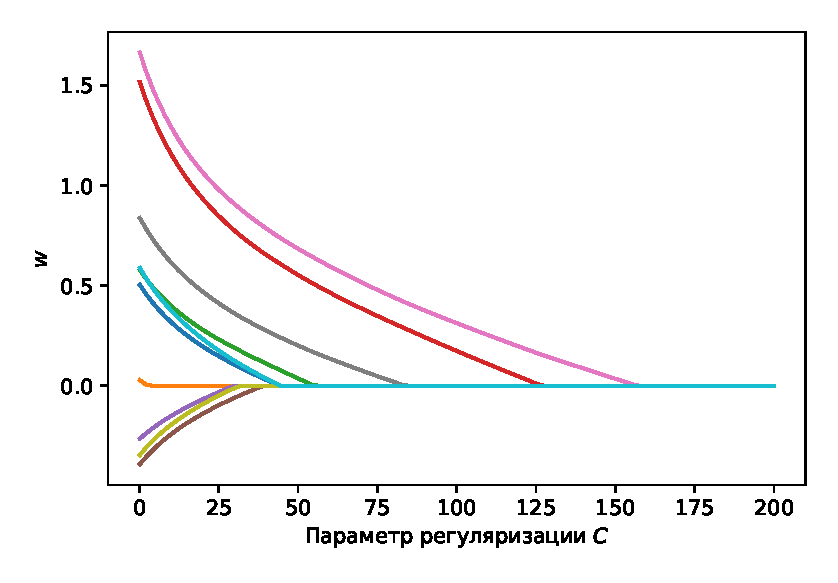
\includegraphics[width=0.5\textwidth]{../figures/log_reg_cs_exp.eps}
% 	\caption{Sample figure caption.}
% 	\label{fig:fig1}
% \end{figure}

% \subsection{Tables}
% See awesome Table~\ref{tab:table}.

% The documentation for \verb+booktabs+ (`Publication quality tables in LaTeX') is available from:
% \begin{center}
% 	\url{https://www.ctan.org/pkg/booktabs}
% \end{center}


% \begin{table}
% 	\caption{Sample table title}
% 	\centering
% 	\begin{tabular}{lll}
% 		\toprule
% 		\multicolumn{2}{c}{Part}                   \\
% 		\cmidrule(r){1-2}
% 		Name     & Description     & Size ($\mu$m) \\
% 		\midrule
% 		Dendrite & Input terminal  & $\sim$100     \\
% 		Axon     & Output terminal & $\sim$10      \\
% 		Soma     & Cell body       & up to $10^6$  \\
% 		\bottomrule
% 	\end{tabular}
% 	\label{tab:table}
% \end{table}

% \subsection{Lists}
% \begin{itemize}
% 	\item Lorem ipsum dolor sit amet
% 	\item consectetur adipiscing elit.
% 	\item Aliquam dignissim blandit est, in dictum tortor gravida eget. In ac rutrum magna.
% \end{itemize}




\bibliographystyle{unsrtnat}
\bibliography{references}

[1] Goemans-Williamson MAXCUT Approximation Algorithm by Jin-Yi Cai, Christopher Hudzik, Sarah Knoop, 2003:
https://pages.cs.wisc.edu/~jyc/02-810notes/lecture20.pdf \\

[2] The Lovasz-Schrijver relaxation by Madhur Tulsiani, 2010: 
https://home.ttic.edu/~madhurt/Papers/ls.pdf \\

% [3] Introduction to the SDP by Robert M. Freund, 2004: https://ocw.mit.edu/courses/15-084j-nonlinear-programming-spring-2004/a632b565602fd2eb3be574c537eea095_lec23_semidef_opt.pdf\\

[4] Treewidth: 
https://www.cs.cmu.edu/~odonnell/toolkit13/lecture17.pdf\\

[5] MAX CUT approximation algorithm and UGC-hardness, Lecture by Irit Dinur and Amey Bhangale:
https://www.wisdom.weizmann.ac.il/~dinuri/courses/19-inapprox/lec6.pdf \\

[6] Semidefinite Programming versus Burer-Monteiro Factorization for Matrix
Sensing by Baturalp Yalcin, Ziye Ma, Javad Lavaei, Somayeh Sojoudi, 2022
https://arxiv.org/abs/2208.07469v1\\

[7] 0.878-approximation for the Max-Cut problem, Lecture by Divya Padmanabhan, 2022: https://www.iitgoa.ac.in/~sreejithav/misc/maxcut.pdf\\

[8] Rank optimality for the Burer-Monteiro factorization by Irène Waldspurger, Alden Waters, 2019 
https://arxiv.org/abs/1812.03046\\

[9] Semidefinite relaxation and nonconvex quadratic optimization by Yury Nesterov, 1997
https://www.tandfonline.com/doi/abs/10.1080/10556789808805690\\

[10] Datasets: Texas Data Repository:
https://dataverse.tdl.org/dataset.xhtml?persistentId=doi:10.18738/T8/VLTIVC\\  

[11] Datasets: Biq Mac Library:
https://biqmac.aau.at/biqmaclib.html\\ 

[12] Datasets: MaxCut and BQP Instance Library:
http://bqp.cs.uni-bonn.de/library/html/index.html\\ 

[13] Datasets: MaxCut Instances:
https://grafo.etsii.urjc.es/optsicom/maxcut.html#best-known-values\\

[14] Ellipsoid algorithm: https://www.cs.toronto.edu/~avner/teaching/S5-2411/ln/lecture8.pdf

[15] Michel X. Goemans and David P. Williamson. Improved approximation algorithms for maximum cut and satisfiability problems using semidefinite programming. Journal of the ACM, 42(6):1115–1145, 1995


\end{document}
